\paragraph{Motivations.\newline}

\etbox{h}{box:intro}{Thermal radiation}{All substances continuously emit electromagnetic radiation by virtue of the molecular and atomic agitation associated with the internal energy of the material. The emitted radiant energy can range from radio waves, which can have wavelengths of tens of meters, to cosmic rays with wavelengths less than $10^{-14}$\,m. In this paragraph we will consider only radiation that is detected as heat. Such radiation is termed \emph{thermal radiation}; it occupies the intermediate frequency range between approximately $10^{-6}$\,m and $10^{-3}$\,m. Radiation from the warm surfaces to the cold surfaces is the dominating mode of heat transfer in vacuum.}

The main heat inputs into the cold mirror of the LF interferometer are the thermal radiation coming from the warm surface of the vacuum tube, and the heat load due to the  absorption of a small fraction of the laser light into the mirror surface. The latter can be estimated considering that the laser power circulating in the optical cavity is 18\,kW, and that a reference value for the absorption coefficient of the mirror optical coating at the working wavelength is around 1\,ppm. This gives an approximate value of 20\,mW of absorbed laser power.

The radiation from the warm surface of the vacuum tube to the mirror can be estimated by the modified Stefan-Boltzmann equation:
\begin{equation}
\label{eq:Stefan-Boltzmann}
\dot{Q_r}/A_1 = \sigma F_e F_{1-2} (T_2^4 - T_1^4)
\end{equation}
where $\dot{Q_r}/A_1$ is the heat transfer rate by radiation per unit area of the mirror surface, $\sigma=5.67\,10^{-8}\, \mathrm{W/m^2/K^4}$ is the Stefan-Boltzmann constant, $F_e$ is the emissivity factor, and $F_{1-2}$ is a geometric configuration factor relating the two surfaces, whose temperatures are $T_2$ (warm) and $T_1$ (cold).  From Eq.~\ref{eq:Stefan-Boltzmann} the heat flux on the mirror at $T_1 = 10$\,K, coming from the vacuum tube at $T_2 = 300$\,K can be as high as $\dot{Q_r}/A_1\sim 460\,\mathrm{W/m^2}$. This huge heat flux is not compatible with the cryogenic environment and needs to be reduced by several orders of magnitude. 

In order to reduce the thermal radiation from the beam duct into the cold mirror, two strategies are viable, as shown by Eq.~\ref{eq:Stefan-Boltzmann}: the reduction of the emissivity factor and/or the reduction of the geometric configuration factor, i.e.\ the reduction of the solid angle under which the warm surface is seen by the cold surface.

The emissivity factor can be reduced by an appropriate choice of material for the wall of the tube, or trough the deposition on the warm surface of a low-emissivity coating. The reduction of the geometric configuration factor, on the other hand, can be obtained by building in the region adjacent to the mirror cold sections of the vacuum tube (thermal shields or cryotraps), that ``move away'' the warm section of the tube from the mirror, and in this way reduce the solid angle under which the warm surface is seen by the cold mirror.  The temperature(s) and length(s) of these sections must be chosen in order to minimize the ration heat transfer to the mirror, and, at the same time, the overall cost of the cryogenic plant. Moreover, they will also serve as cryogenic pumps. In particular, in the region immediately adjacent to the mirror, a zone \emph{colder} than the mirror itself is needed to avoid the condensation of the residual gas on the surface of the mirror, that could lead to the growth of a layer of contaminants and spoil its optical characteristics.
 
\paragraph{Maximum heat load on cryogenic mirror.\newline}

The equilibrium temperature of the mirror is reached when the power extracted by the cooling system is equal to the power absorbed by the mirror ($\dot{Q}_{abs}=\dot{Q}_{coolsys}$). The power extracted by the cooling system mostly flows through the four silicon suspension wires (a small fraction is exchanged with the surroundings through thermal radiation) to the penultimate mass (the marionette) and then is removed by the heat sink directly connected to the cooling system.
The equilibrium temperature of the mirror $T_{mir}$ can be calculated by a simple analytical model if we assume that the temperature of the penultimate mass is kept fixed at the design value of 5\,K:
\begin{eqnarray}
\dot Q_{abs} & =  & \frac{4  S_w}{L}<k_{Si}>\left (T_{mir} - T_{mario}\right) \\
 <k_{si}> & = & \frac{1} {{\Delta T}}\int\limits_{T_{mir}}^{T_{mario}} {{k_{si}}(T)_{}^{}dT}
\end{eqnarray}
where $S_w$ is the section of the silicon suspension wire, $L$ is its length and $k_{si}(T)$ is the thermal conductivity of silicon. In the following calculations we shall use the thermal conductivity shown in Fig.~\ref{fig:k-silicon-comsol}~\cite{k-silicon-comsol}. From this figure we see that $<k_{si}>\sim 1.4\, 10^3 \, \mathrm{W/m/K}$  in the temperature range of interest (5--10\,K). We also take the design values for the silicon suspension wires (diameter: 3\,mm, length: 2\,m). The maximum power that can be extracted from the mirror, keeping its temperature at the design value of 10\,K, is approximately 100\,mW. 
\begin{figure}[htbp]
	\begin{center}
		 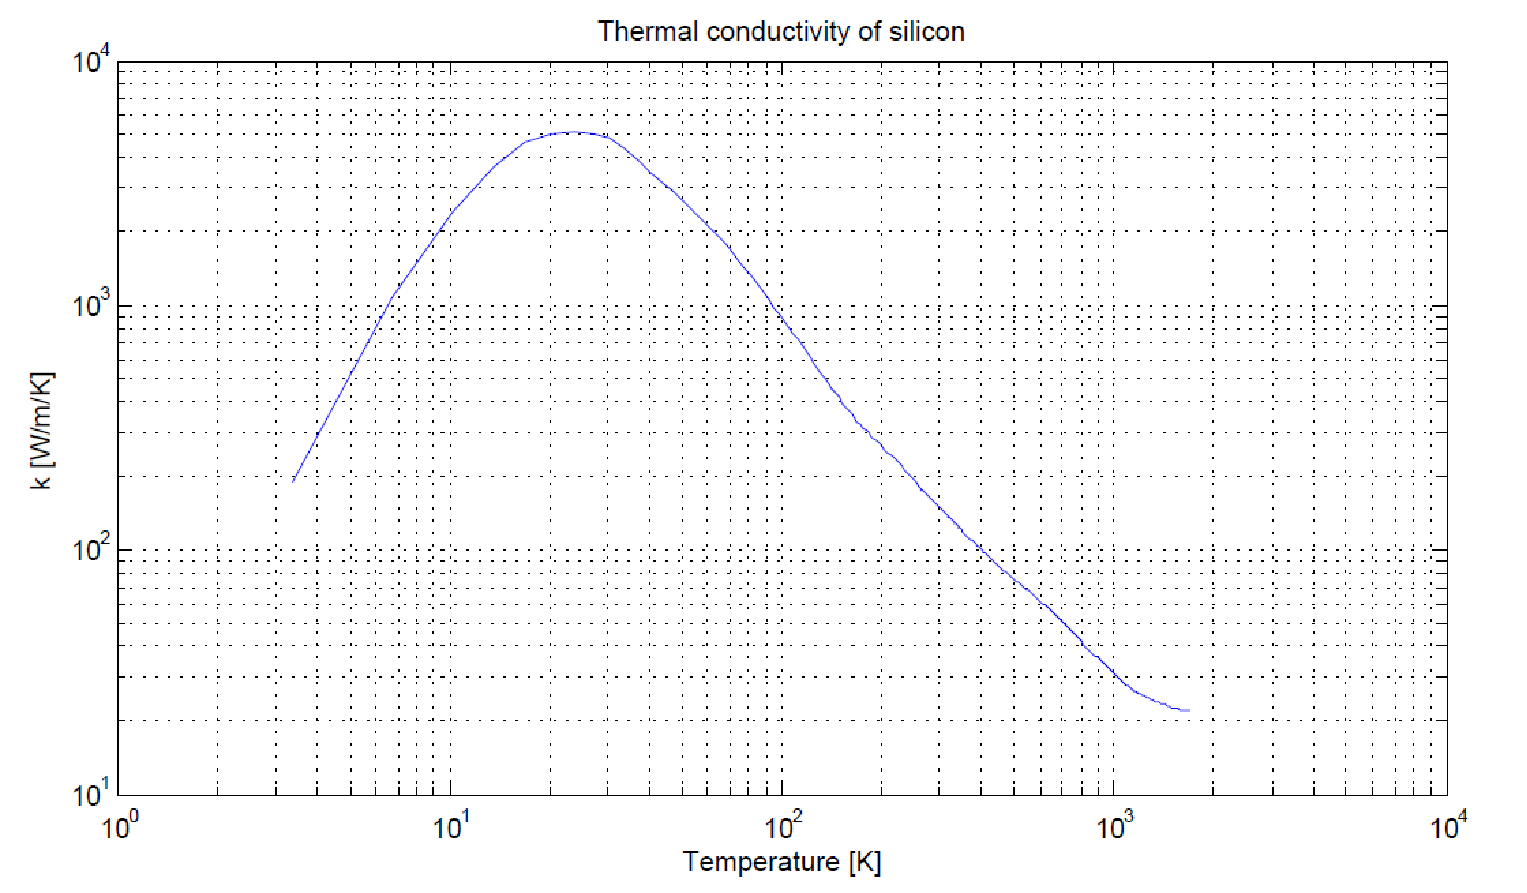
\includegraphics[width=12cm]{Sec_SiteInfra/Cryotraps/k-silicon-comsol.pdf}
			\caption{Thermal conductivity of silicon  (from \cite{k-silicon-comsol})}		
			\label{fig:k-silicon-comsol}
	\end{center}
\end{figure}
Since the laser power absorbed by the mirror is approximately 20\,mW, we can conclude that the thermal radiation heat load must not exceed $\sim$ 80\,mW.

%\paragraph{Heat load on cryogenic mirror -- finite element model.}
The above back-of-the-envelope calculation was checked by a finite element model of the mirror and its suspension system, as shown in Fig.~\ref{fig:model}
\begin{figure}[htbp]
\begin{center}
 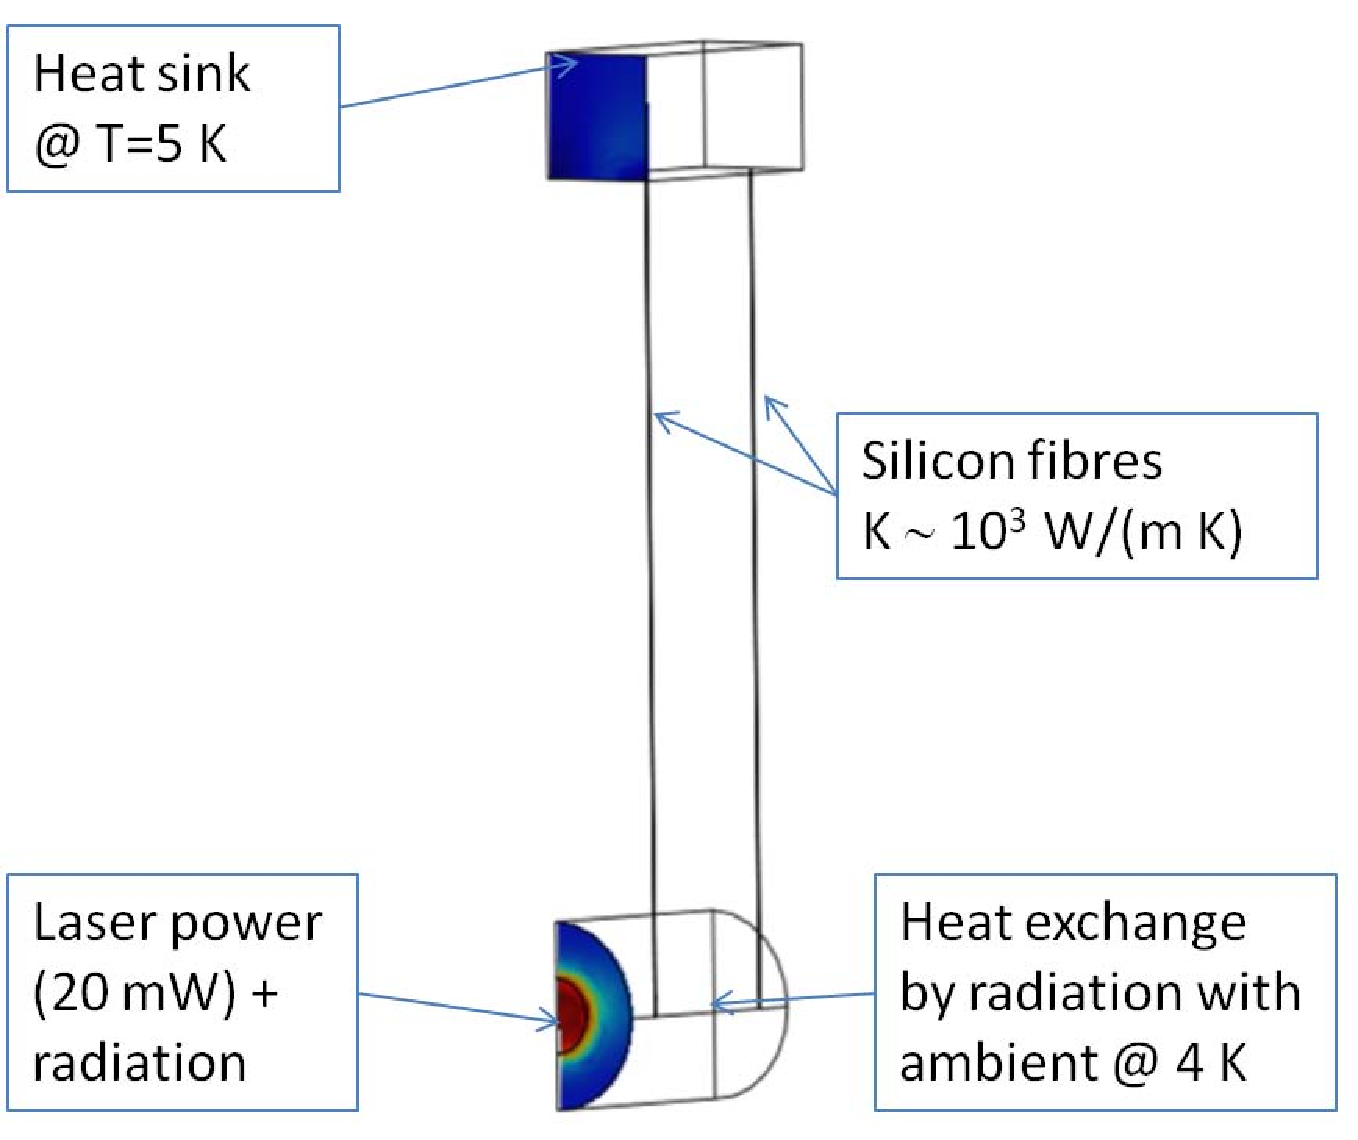
\includegraphics[width=12cm]{Sec_SiteInfra/Cryotraps/model.pdf}
			\caption{Finite element model and boundary conditions}
\label{fig:model}
\end{center}
\end{figure}
The parameters used in the model are summarized in table~\ref{tab:model-parameters}.
\begin{table}[htbp]
\caption{Finite element model parameters}
\begin{center}
\begin{tabular}{|l|l|}
\hline \rule[-2ex]{0pt}{5.5ex} Mirror temperature & 10\,K \\ 
\hline \rule[-2ex]{0pt}{5.5ex} Mirror diameter & 45\,cm \\ 
\hline \rule[-2ex]{0pt}{5.5ex} Mirror mass & 211\,Kg \\ 
\hline \rule[-2ex]{0pt}{5.5ex} Silicon fibers length & 2\,m \\ 
\hline \rule[-2ex]{0pt}{5.5ex} Silicon fibers diameter & 3\,mm \\ 
\hline \rule[-2ex]{0pt}{5.5ex} Marionette temperature & 5\,K \\ 
\hline \rule[-2ex]{0pt}{5.5ex} Power in cavity & 18\,kW \\ 
\hline \rule[-2ex]{0pt}{5.5ex} Absorbed power  & 20\,mW \\ 
\hline \rule[-2ex]{0pt}{5.5ex} Beam radius & 9\,cm \\ 
\hline 
\end{tabular} 
\end{center}
\label{tab:model-parameters}
\end{table}

The calculation was done setting on the front surface of the mirror a fixed heat source, representing the power coming from the laser and absorbed by the mirror, of 20\,mW, with superimposed a variable heat source, representing the additional heat load due to thermal radiation. For the sake of simplicity the temperature of the penultimate mass was set at the fixed value of 5\,K.  The thermal conductivity of silicon shown in Fig.~\ref{fig:k-silicon-comsol} was used in the model~\cite{k-silicon-comsol}.

The solution of the problem was calculated sweeping the variable heat source in the 0--0.1\,W range, with steps of 10\,mW, and looking at the temperature in the central area of the mirror. The results are shown in Fig.~\ref{fig:T-mirror-0-100}. They confirm the order-of-magnitude values found in the previous section. The temperature of the central area of the mirror does not exceed 10\,K when the thermal radiation is lower than 70\,mW, corresponding to 90\,mW of total power absorbed by the mirror.
\begin{figure}[htbp]
\begin{center}
 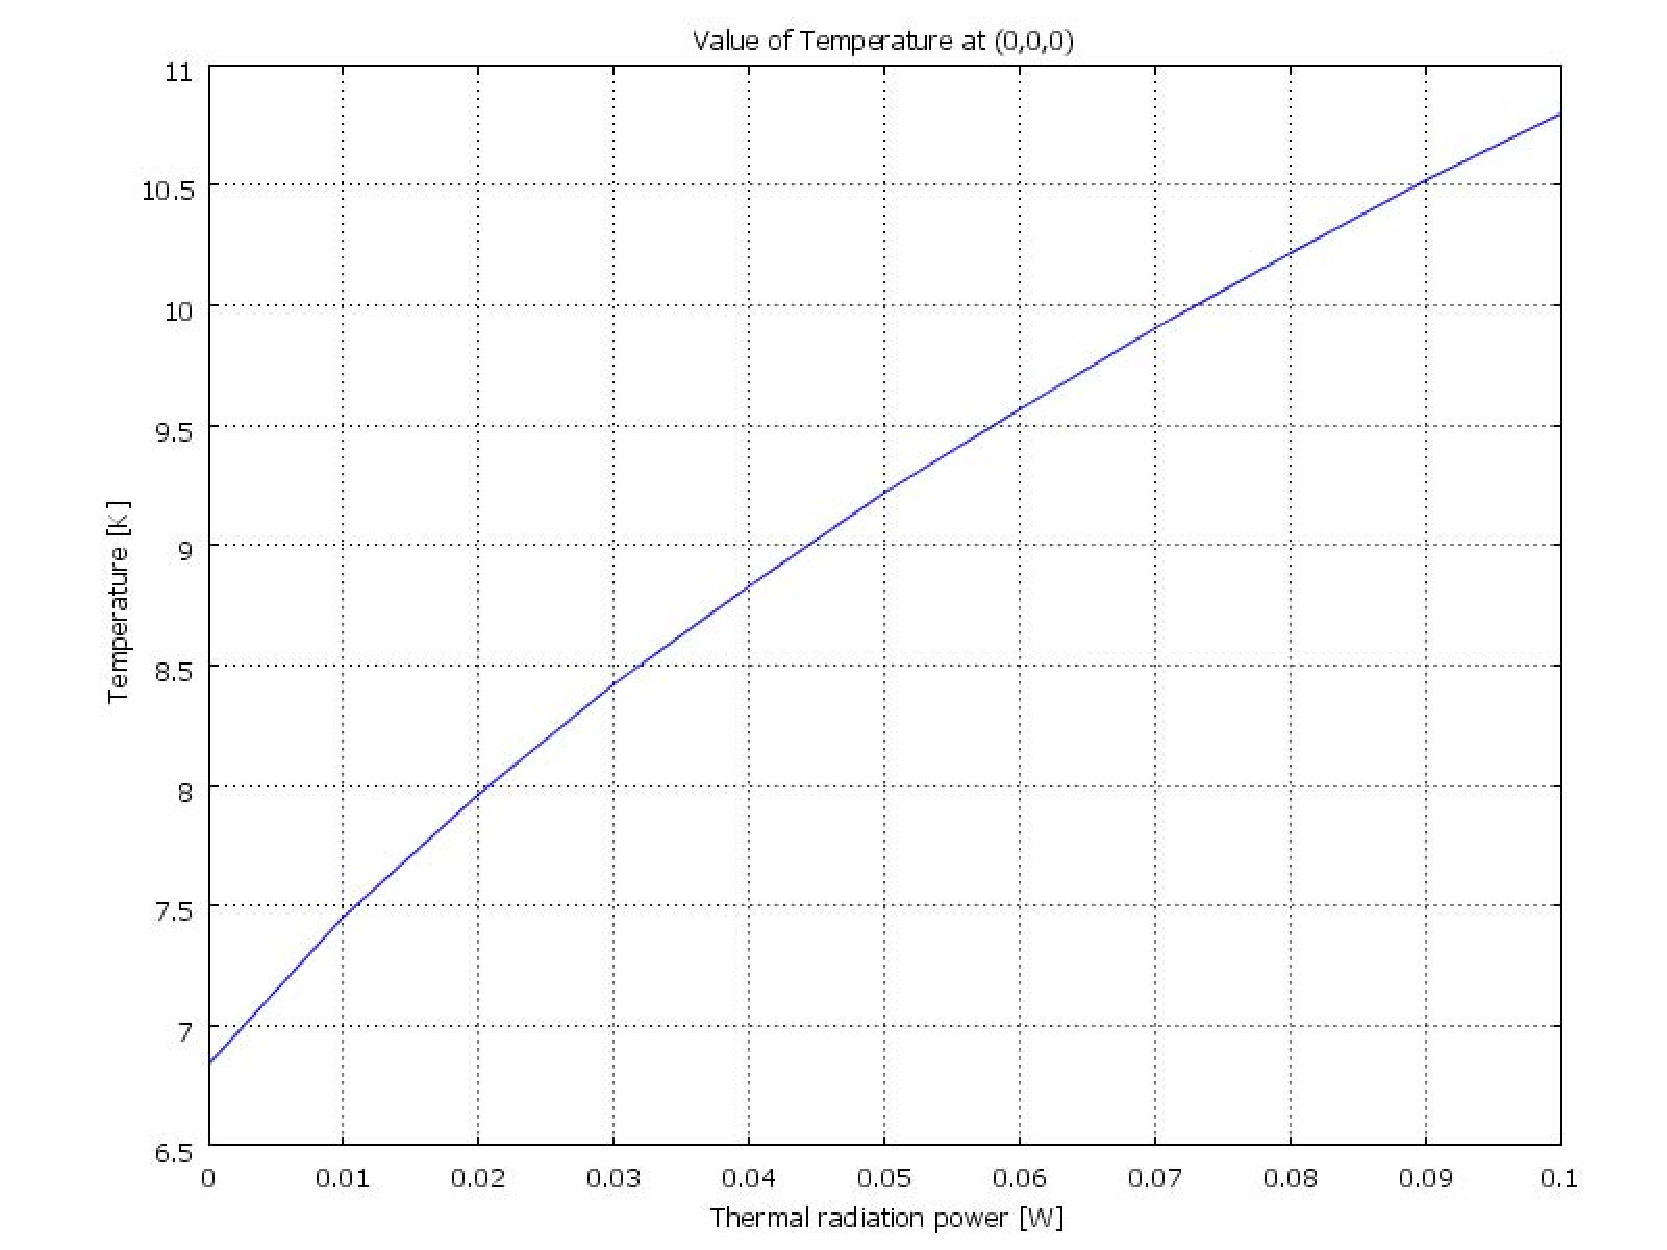
\includegraphics[width=12cm]{Sec_SiteInfra/Cryotraps/T_mirror-0-100.pdf}
			\caption{Temperature at the center of the mirror vs.\ thermal radiation power}
\label{fig:T-mirror-0-100}
\end{center}
\end{figure}

\etbox{r}{box:maxpower}{Maximum thermal radiation power on cold mirror}{The maximum power that the mirror can absorb, keeping its temperature at the fixed value of 10\,K is approximately 90\,mW. Since the power absorbed from the laser is 20\,mW, the thermal radiation power must not exceed 70\,mW. In order to reduce the thermal radiation from the beam duct into the cold mirror, two strategies are viable: the reduction of the emissivity factor and/or the reduction of the geometric configuration factor, i.e.\ the reduction of the solid angle under which the warm surface is seen by the cold surface. The reduction of the geometric configuration factor can be obtained by building in the region adjacent to the mirror cold sections of the vacuum tube, that ``move away'' the warm section of the tube from the mirror, and in this way reduce the solid angle under which the warm surface is seen by the cold mirror.} 

In the following paragraph we shall find out how to design the thermal shields in the region adjacent to the mirror to keep the thermal radiation from the warm surface of the vacuum tube at a value not greater than few tens of milliwatts.

\paragraph{Thermal radiation from vacuum tubes - Direct exchange. \newline}

Radiative transfer of heat from one area to another depends, among
other things, upon the fraction of the radiant energy emitted by one area
which is intercepted by a second area. This fraction is identified by
several names, such as the configuration factor, the interchange factor,
the angle factor, or the geometric view factor, and is a function of the
geometrical relation of the areas involved. The configuration factor is defined as the fraction of diffusely radiated energy leaving surface A that is incident on surface B, and it is represented by the $F_{1-2}$ factor that appears in Eq.~\ref{eq:Stefan-Boltzmann}. 

We have to explicitly calculate the configuration factor for the geometry schematically shown in Fig.~\ref{fig:vacuum-tube}
\begin{figure}[htbp]
\begin{center}
 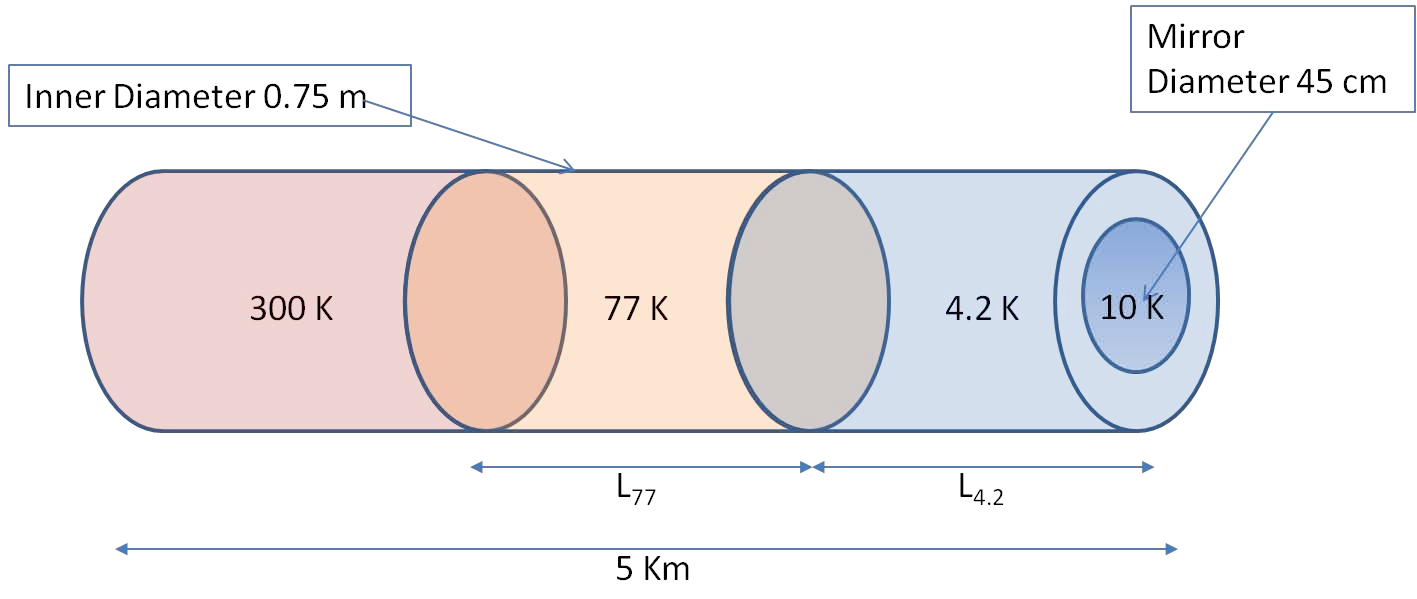
\includegraphics[width=12cm]{Sec_SiteInfra/Cryotraps/vacuum-tube.pdf}
			\caption{Conceptual scheme of the vacuum tube with cryotraps}
\label{fig:vacuum-tube}
\end{center}
\end{figure}

The details of the calculation are presented in Appendix~\ref{sec:geometric-appendix}. Making use of Eq.~\ref{eq:Stefan-Boltzmann} we can calculate the thermal radiation power on the mirror as a function of the lengths of the two cold sections, at 4.2\,K and 77\,K. The result is shown in Fig.~\ref{fig:contour}
\begin{figure}[htbp]
\begin{center}
 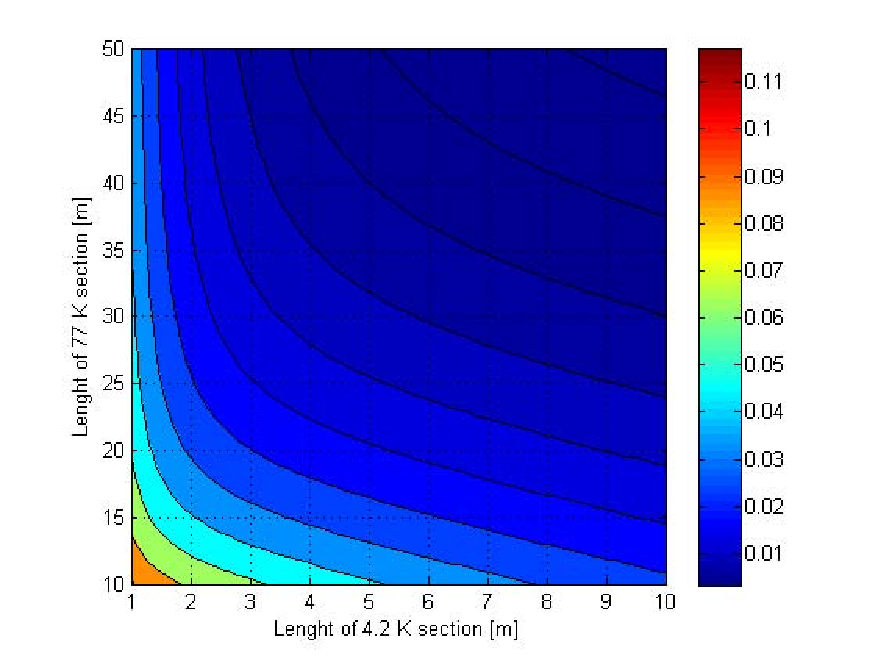
\includegraphics[width=12cm]{Sec_SiteInfra/Cryotraps/contour.pdf}
			\caption{Thermal radiation on the mirror vs.\ lengths of 4.2\,K and 77\,K sections.}
\label{fig:contour}
\end{center}
\end{figure}

\etbox{r}{box:cryolength}{Lenghts of the cryotraps}{We see that to keep the thermal radiation power in the range $\sim 10$\,mW, we need a 4.2\,K section of few meters and a 77\,K section of few tens of meters. For example, with $L_{4.2}=10$\,m and $L_{77}=50$\,m, we are in a situation were the \emph{direct} transfer of thermal energy from the warm tube to the mirror is approximately 3\,mW, well below the maximum allowed value.}

\paragraph{Thermal radiation from vacuum tubes - specular and diffuse reflection.\newline}
\etbox{h}{box:specdiff}{Specularly and diffusely reflecting surfaces}{The calculation of the thermal energy \emph{directly} transferred from the warm surface to the cold mirror is not sufficient. For the correct evaluation of the thermal radiation on the cold mirror reflections along the cryo-shields including the reflective properties of the surfaces must be taken into account.  These are rather difficult to specify as the reflected energy depends not only on the angle at which the incident energy impinges on the surface but also on the direction being considered for the reflected energy.  Two important, and relatively simple, limiting cases can be used for calculating heat exchange: \emph{diffuse} surfaces and \emph{specular} surfaces. In specular reflection, also called mirror like reflection, the propagation direction of the radiation is not significantly changed, whereas in the case of diffuse reflection the reflected radiation is reflected into all directions. An ideally diffusely reflecting surface will have will equal luminance for all directions.}

For a diffuse surface the incident energy from the direction $(\theta, \phi)$ that is reflected produces a reflected intensity that is uniform over all $(\theta_r, \phi_r)$ directions. When a diffuse surface element irradiated by an incident beam is viewed, the element appears equally bright from all viewing directions.  In the previous paragraphs, all the surfaces involved in the calculation of the configuration factors---in particular the inner surface of the vacuum tube---were assumed to be diffuse emitters.

Mirror-like, or specular, surfaces obey well-known laws of reflection. For an incident beam from a single direction, in a specular reflector, the reflected beam is at the same angle away from the surface normal as the incident beam, and is in the same plane as that formed by the incident beam and surface normal. When reflection is diffuse, the directional history of the incident radiation is lost upon reflection. With specular reflection the directional history of the incident radiation is not lost upon reflection. Consequently, when dealing with specular surfaces, it is necessary to account for the specific directional paths that the reflected radiation follows between surfaces.

An important parameter for deciding whether a surface falls in the diffuse or specular limit is the surface roughness, or more precisely the ratio of the root-mean-square roughness to the wavelength of the radiation. For long-wavelength radiation a smooth surface tends toward being optically smooth, and the reflections tend to become more specular. Thus, although a surface may not appear mirror-like to the eye (i.e.\ for the short wavelengths of the visible spectrum), it may be specular for longer wavelengths in the infrared.

The contribution to the thermal radiation heat transfer coming from \emph{diffuse} reflectivity was calculated for the geometry given in Fig.~\ref{fig:vacuum-tube} by a finite-element model (for the details see Appendix~\ref{sec:diffuse-appendix}). The geometric dimensions of the system were the same as in table~\ref{tab:model-parameters}, with the lengths of the cold sections $L_{77}= 50$\,m and  $L_{4.2}= 10$\,m. The results are shown in Fig.~\ref{fig:q_eps_diffuse}:
\begin{figure}[htbp]
\begin{center}
 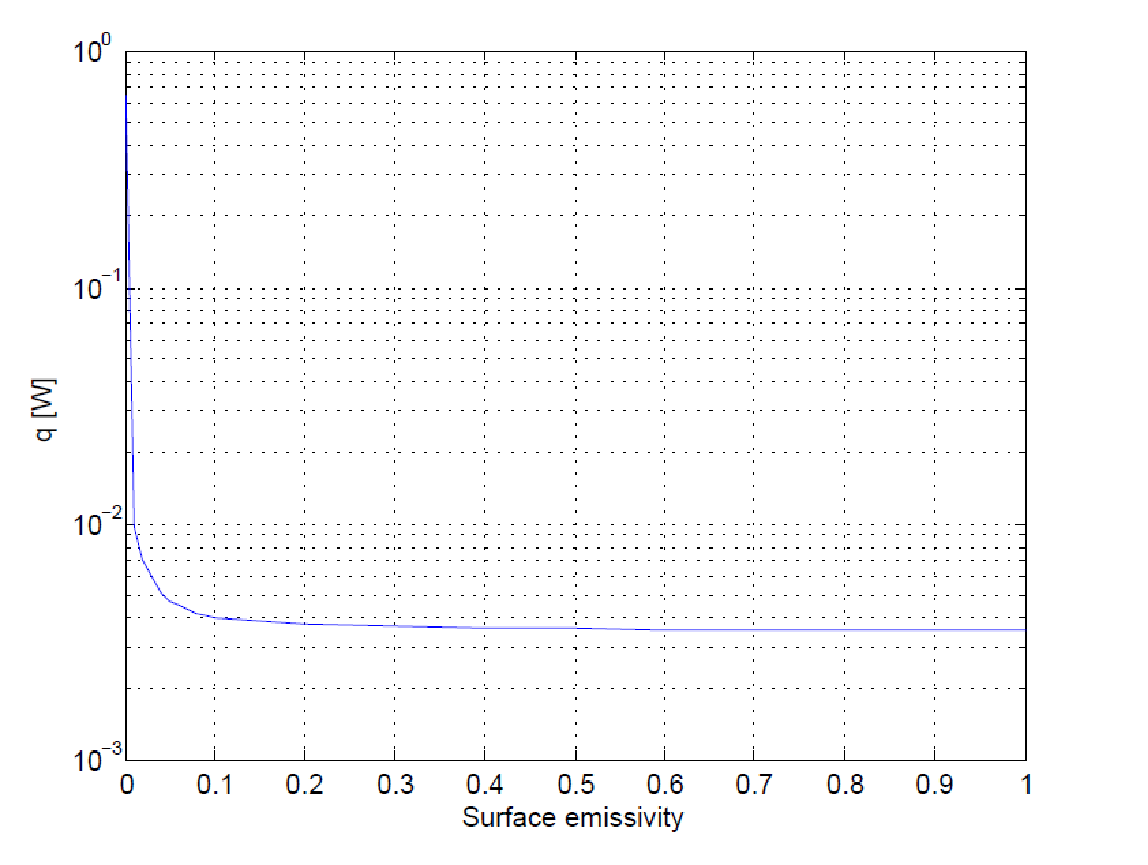
\includegraphics[width=11cm]{Sec_SiteInfra/Cryotraps/q_eps_diffuse.pdf}
			\caption{Thermal radiation heat transfer in the diffuse reflection limit}
\label{fig:q_eps_diffuse}
\end{center}
\end{figure}

The case when the pipe walls are specularly reflecting was discussed in~\cite{tomaru_2007, tomaru_2008}. A large heat load caused by thermal radiation through a metal shield pipe was observed in a cooling test of a cryostat for a prototype of the cryogenic
interferometric gravitational wave detector (CLIO) in Japan. The heat load was approximately
three orders of magnitude larger than the value calculated by the Stefan-Boltzmann law. The phenomenon was studied both by simulation and by experiment and it was found that found that it was caused by the conduction of thermal radiation in a metal shield pipe due to multiple specular reflections in the pipe. 

A simple model for the evaluation is illustrated in Fig.~\ref{fig:specular}~\cite{mosher_1976}.
\begin{figure}[htbp]
\begin{center}
 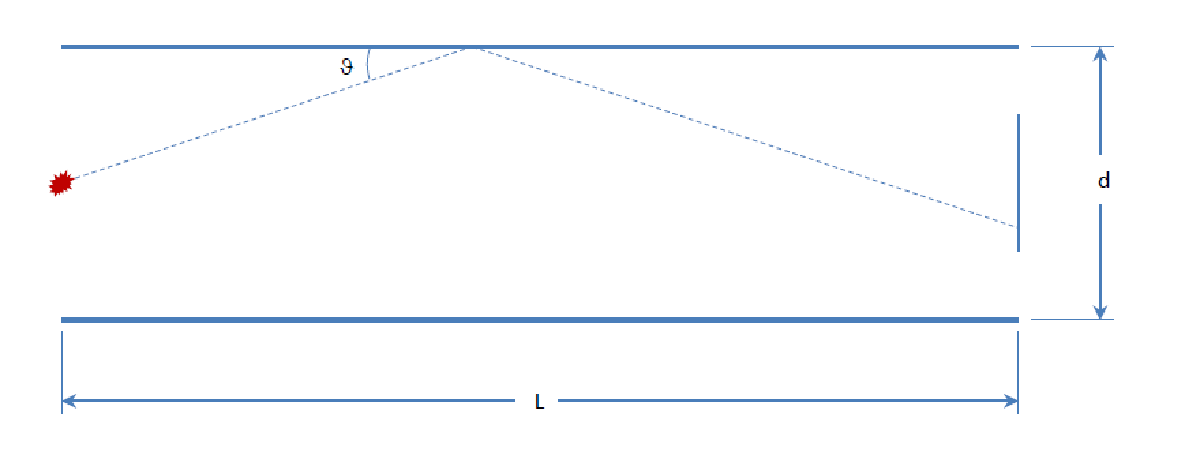
\includegraphics[width=11cm]{Sec_SiteInfra/Cryotraps/specular.pdf}
			\caption{Thermal radiation "light-pipe" geometry for an on-axis source}
\label{fig:specular}
\end{center}
\end{figure}

In the case we are considering the aspect ratio of the pipe is sufficiently large to make the number of reflections
\begin{equation}
N \sim \frac{L}{d} \tan \theta	
\end{equation}
a number large compared to unity. At each reflection the radiation intensity is reduced by an amount $\rho(\theta)=1-\epsilon$ the specular reflection coefficient of the wall. The total reduction in intensity due to reflections at a given angle of incidence in the tube is determined by $\rho^N$.

The efficiency of transfer of radiation, $\eta$ emitted by an on-axis point source is then
\begin{equation}
\eta = \int_0^{\frac{\pi}{2}} \rho^N \sin \theta \, d\theta
\end{equation}
The plot of the radiation heat transferred to the mirror by specular radiation is shown in Fig.~\ref{fig:q_eps_specular}.
\begin{figure}[htbp]
\begin{center}
 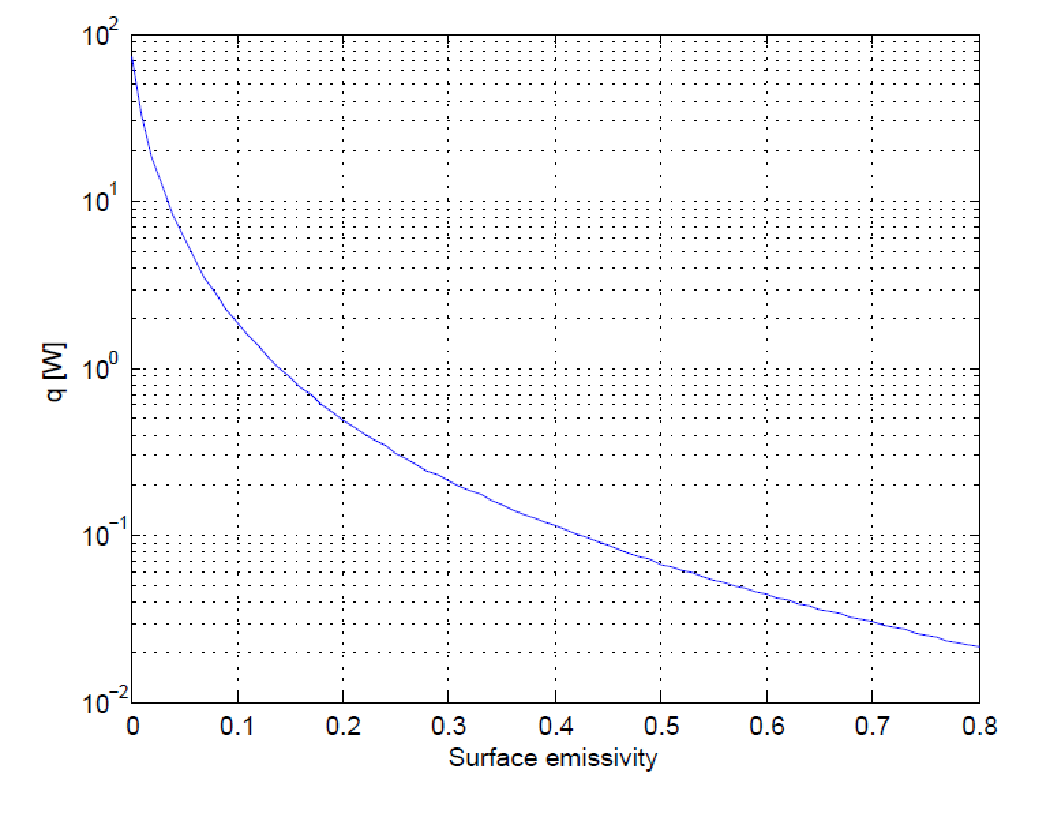
\includegraphics[width=10cm]{Sec_SiteInfra/Cryotraps/q_eps_specular.pdf}
			\caption{Thermal radiation heat transfer in the specular reflection limit}
\label{fig:q_eps_specular}
\end{center}
\end{figure}

\etbox{r}{box:diffheat}{Heat transfer from diffusely and specularly reflecting surfaces}{We see that for $\epsilon \geq 0.1$ the heat transferred to the mirror is essentially the direct contribution from the warm tube. Only for small values of $\epsilon < 0.1$ (high reflectivity $\delta > 0.9$) the contribution to the heat transfer from the surface reflectivity increases dramatically. On the other hand, we see that for specularly reflecting surfaces a huge amount of heat reaches the mirror for almost all the values of the emissivity. Specular reflections inside the vacuum pipe must be strongly suppressed.}

\paragraph{Mitigation strategies.\newline}
\begin{itemize}
\item{The \emph{direct} radiation heat from the tube at 300\,K to the cold mirror is strongly suppressed with cold sections (cryogenic shields, or cryotraps) near the mirror. With a section 10\, m long, cooled at liquid helium temperature, and a section 50\, m long, cooled at liquid nitrogen temperature, the direct heat transfer can be reduced in the milliwatt range.}
\item{For the given cold pipe aspect ratio $L/d \sim 80$, the contribution of \emph{diffuse} reflectivity of the surface of the cold sections becomes important only for reflectivity $\delta > 0.9$ ($\epsilon < 0.1$).}
\item{Specular reflection in the cryogenic shields can increase the radiation heat transfer by two or three orders of magnitude. The effect can be controlled by placing absorbing baffles on the radiation paths inside the cold pipe; by coating the inner surface of the cold pipe with an high emissivity layer ($\epsilon > 0.9$); increasing the surface roughness of the cold pipe to suppress the mirror-like reflections} 
\end{itemize}
